\begin{figure}[ht]
\centering
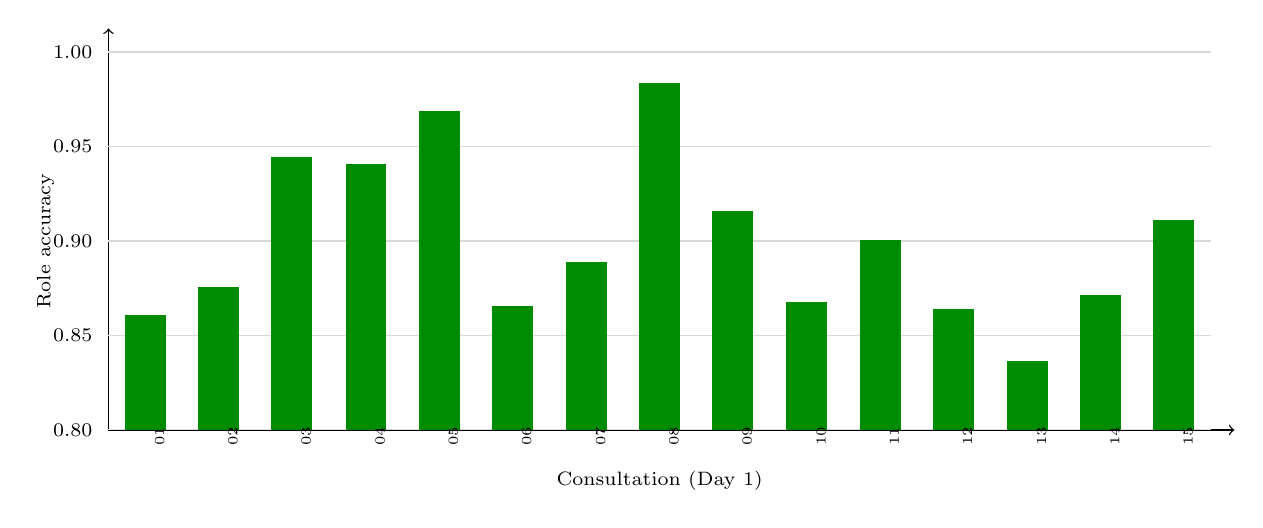
\begin{tikzpicture}[x=1cm,y=1cm]
\draw[->, line width=0.5pt] (1.00,0.80) -- (1.00,5.90);
\draw[->, line width=0.5pt] (1.00,0.80) -- (15.30,0.80);
\draw[gray!30] (1.00,0.80) -- (15.00,0.80);
\node[anchor=east,font=\scriptsize] at (0.92,0.80) {0.80};
\draw[gray!30] (1.00,2.00) -- (15.00,2.00);
\node[anchor=east,font=\scriptsize] at (0.92,2.00) {0.85};
\draw[gray!30] (1.00,3.20) -- (15.00,3.20);
\node[anchor=east,font=\scriptsize] at (0.92,3.20) {0.90};
\draw[gray!30] (1.00,4.40) -- (15.00,4.40);
\node[anchor=east,font=\scriptsize] at (0.92,4.40) {0.95};
\draw[gray!30] (1.00,5.60) -- (15.00,5.60);
\node[anchor=east,font=\scriptsize] at (0.92,5.60) {1.00};
\fill[green!55!black] (1.21,0.80) rectangle (1.73,2.26);
\node[anchor=north,font=\tiny,rotate=90] at (1.47,0.72) {01};
\fill[green!55!black] (2.14,0.80) rectangle (2.66,2.61);
\node[anchor=north,font=\tiny,rotate=90] at (2.40,0.72) {02};
\fill[green!55!black] (3.07,0.80) rectangle (3.59,4.27);
\node[anchor=north,font=\tiny,rotate=90] at (3.33,0.72) {03};
\fill[green!55!black] (4.01,0.80) rectangle (4.53,4.18);
\node[anchor=north,font=\tiny,rotate=90] at (4.27,0.72) {04};
\fill[green!55!black] (4.94,0.80) rectangle (5.46,4.85);
\node[anchor=north,font=\tiny,rotate=90] at (5.20,0.72) {05};
\fill[green!55!black] (5.87,0.80) rectangle (6.39,2.37);
\node[anchor=north,font=\tiny,rotate=90] at (6.13,0.72) {06};
\fill[green!55!black] (6.81,0.80) rectangle (7.33,2.93);
\node[anchor=north,font=\tiny,rotate=90] at (7.07,0.72) {07};
\fill[green!55!black] (7.74,0.80) rectangle (8.26,5.20);
\node[anchor=north,font=\tiny,rotate=90] at (8.00,0.72) {08};
\fill[green!55!black] (8.67,0.80) rectangle (9.19,3.58);
\node[anchor=north,font=\tiny,rotate=90] at (8.93,0.72) {09};
\fill[green!55!black] (9.61,0.80) rectangle (10.13,2.42);
\node[anchor=north,font=\tiny,rotate=90] at (9.87,0.72) {10};
\fill[green!55!black] (10.54,0.80) rectangle (11.06,3.21);
\node[anchor=north,font=\tiny,rotate=90] at (10.80,0.72) {11};
\fill[green!55!black] (11.47,0.80) rectangle (11.99,2.33);
\node[anchor=north,font=\tiny,rotate=90] at (11.73,0.72) {12};
\fill[green!55!black] (12.41,0.80) rectangle (12.93,1.68);
\node[anchor=north,font=\tiny,rotate=90] at (12.67,0.72) {13};
\fill[green!55!black] (13.34,0.80) rectangle (13.86,2.51);
\node[anchor=north,font=\tiny,rotate=90] at (13.60,0.72) {14};
\fill[green!55!black] (14.27,0.80) rectangle (14.79,3.46);
\node[anchor=north,font=\tiny,rotate=90] at (14.53,0.72) {15};
\node[rotate=90,font=\scriptsize] at (0.20,3.20) {Role accuracy};
\node[font=\scriptsize] at (8.00,0.15) {Consultation (Day 1)};
\end{tikzpicture}
\caption{Per-consultation Step~4 speaker-role accuracy computed by overlap between predicted transcript segments and PriMock57 doctor/patient TextGrid intervals.}
\label{fig:consultation-role-accuracy}
\end{figure}
